\subsection{Архитектура}
    Программный комплекс состоит из набора подсистем, которые выполняют набор функций:
    \begin{enumerate}
        \item получение данных из твиттера;
        \item получение данных из новостной rss-ленты;
        \item расшифровка коротких URL;
        \item автоматическое построение набора данных;
        \item построение набора данных на основе вручную построенных заготовок;
        \item построение моделей для методов WTMF и WTMF-G;
        \item построение рекомендаций для методов WTMF, WTMF-G и поиска схожести на основе частнотности употребления слов;
        \item оценка качества рекомендаций;
        \item получение результатов рекомендаций в пригодном для чтения формате;
    \end{enumerate}

    подробное описание архитектуры системы приведённой на flowchart

    \begin{sidewaysfigure}[h!]
            \center
            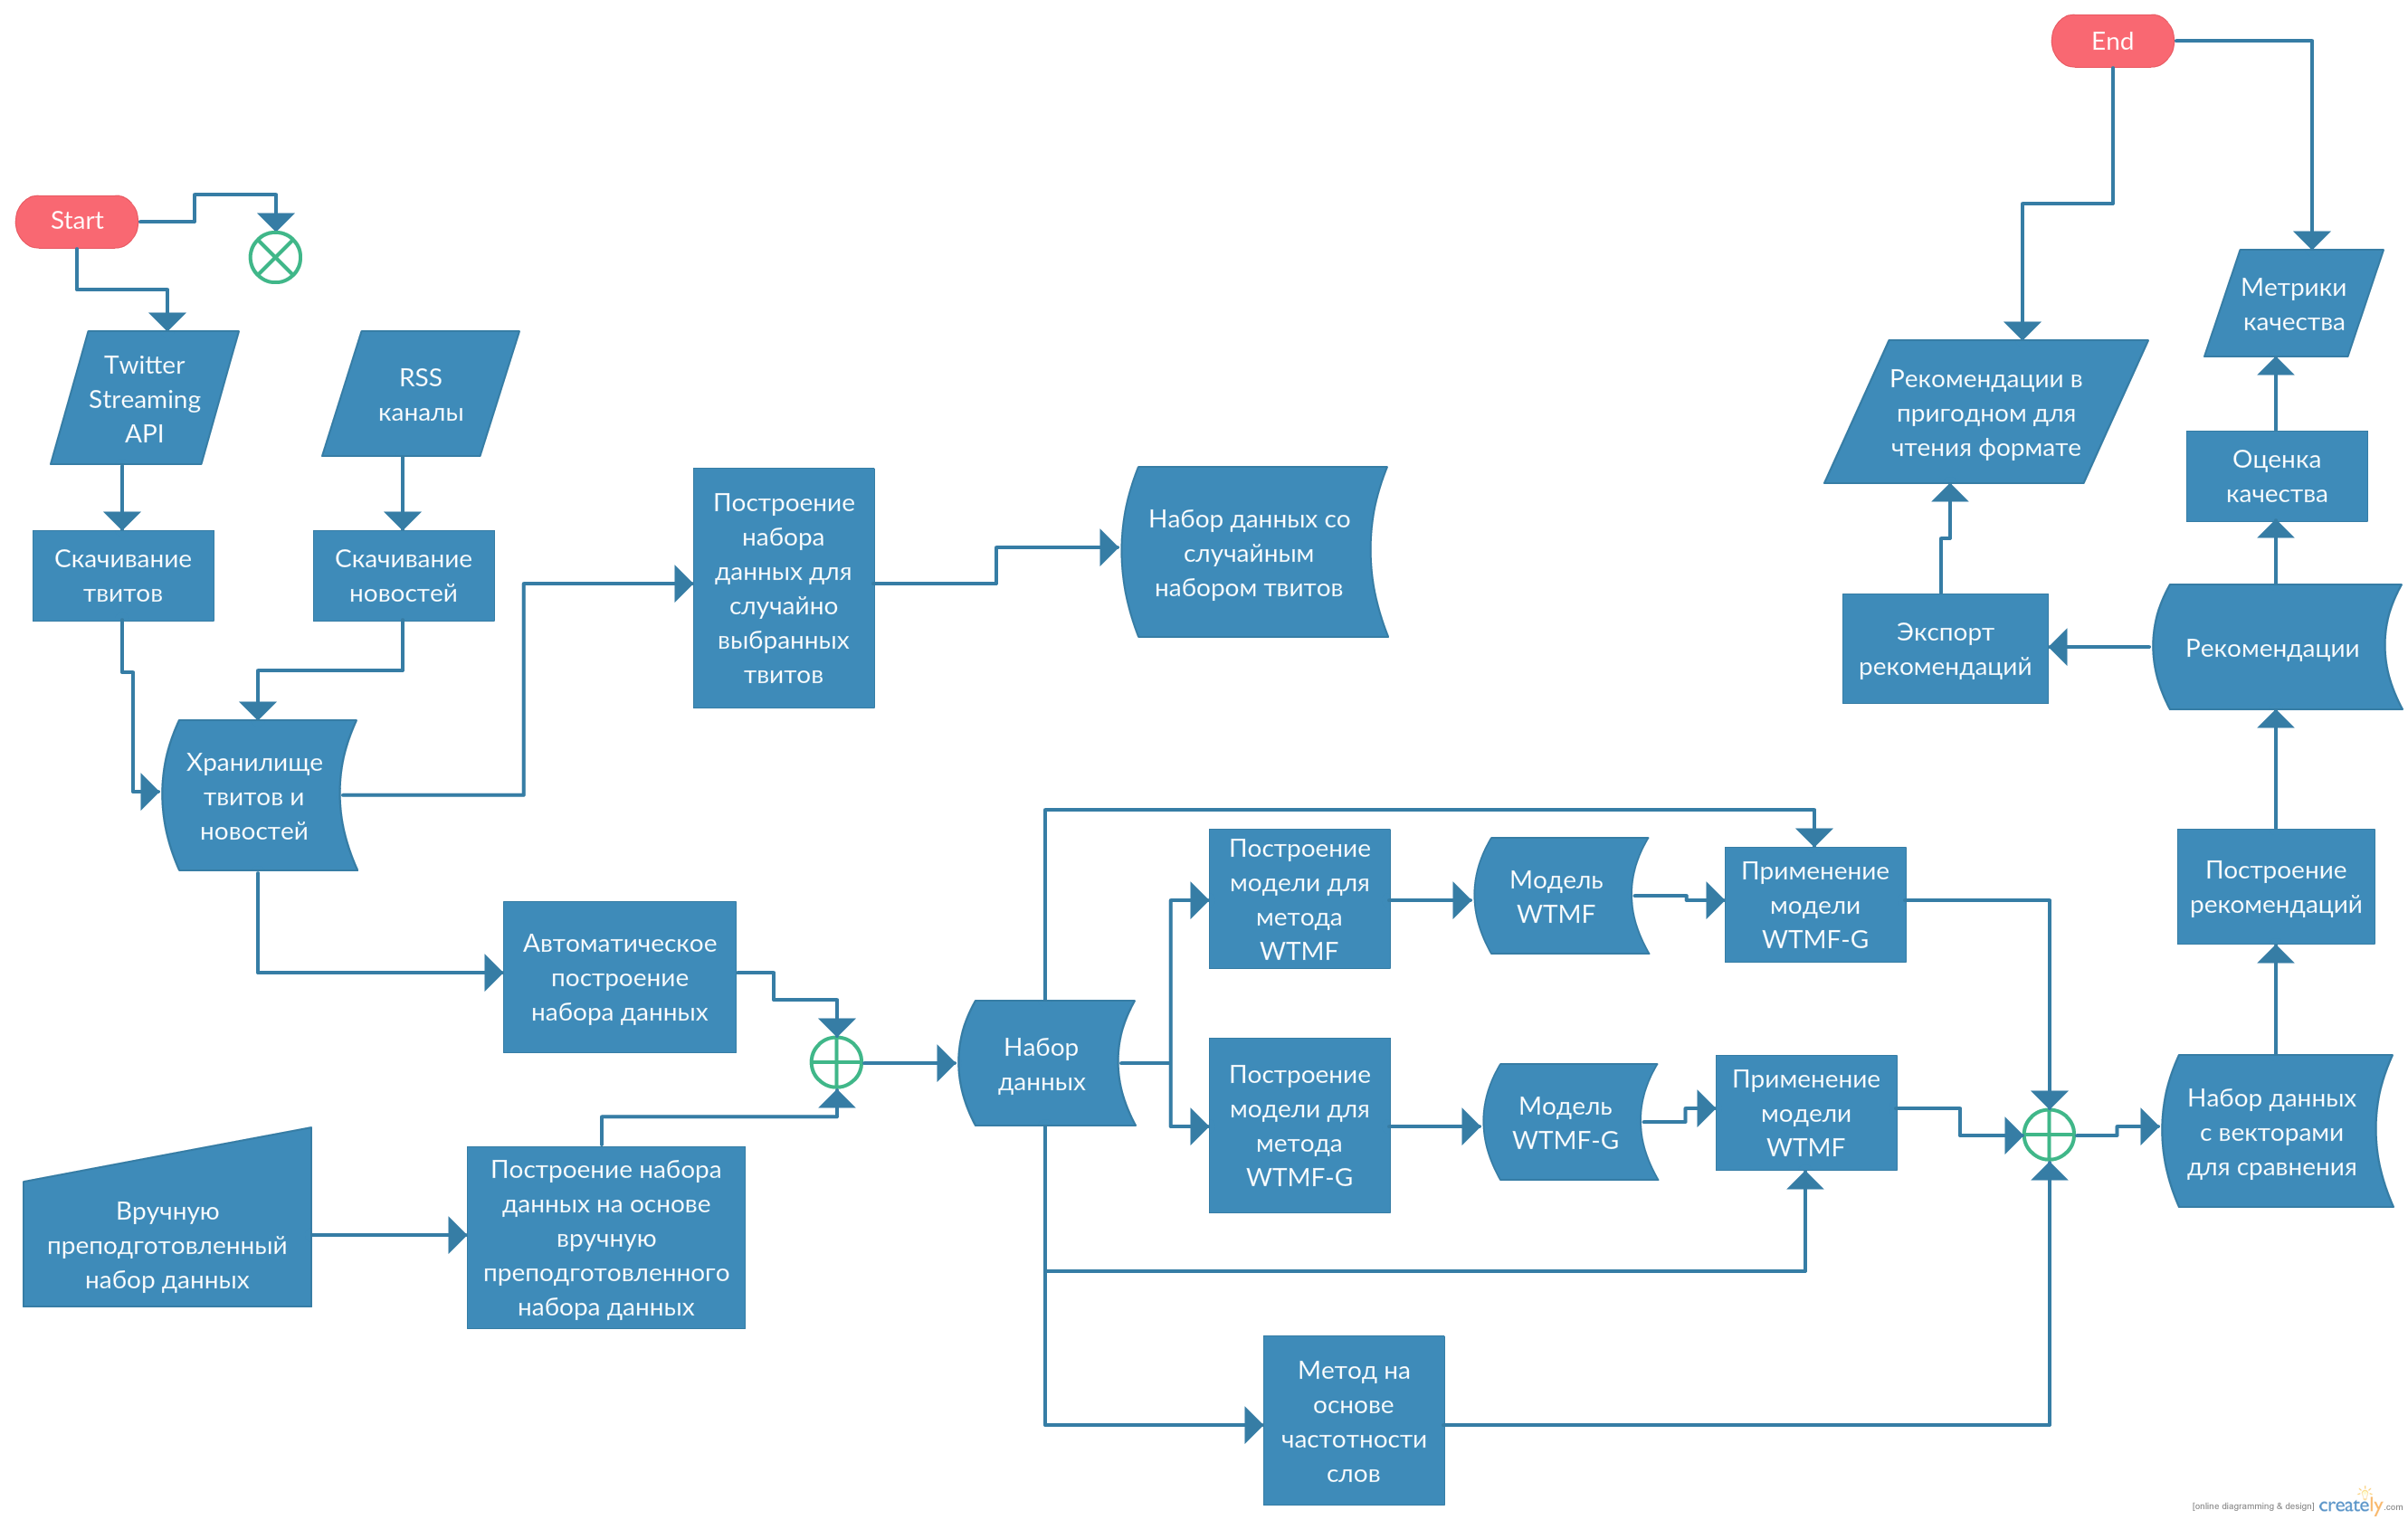
\includegraphics[scale=0.25]{twnews_flowchart.png}
            \caption{flow chart}
            \label{pic:flowchart}
    \end{sidewaysfigure}

    \clearpage



